\documentclass{article}

% set font encoding for PDFLaTeX, XeLaTeX, or LuaTeX
\usepackage{ifxetex,ifluatex}

\if\ifxetex T\else\ifluatex T\else F\fi\fi T%
  \usepackage{fontspec}
\else
  \usepackage[T1]{fontenc}
  \usepackage[utf8]{inputenc}
  \usepackage{lmodern}
\fi

\usepackage{amsmath}
\usepackage{amssymb}
\usepackage{amsthm}
\usepackage{bm}
\usepackage{mathtools}
\usepackage{physics}

\usepackage{enumitem}
\usepackage{multicol}
\usepackage{graphicx}

\usepackage{hyperref}
\hypersetup{colorlinks=true,}
\usepackage[parfill]{parskip}
\usepackage{lipsum}
\usepackage[export]{adjustbox}
\usepackage{listings}

\usepackage{xparse} 
\usepackage{subfig} 
\usepackage{xparse} 
\usepackage{float}

\usepackage{biblatex} 

%%%%%This is an image table command, can likely be deleted
\newcommand{\subf}[2]{

%
{\small 
\begin{tabular}
  [t]{@{}c@{}} #1\ 
  \#2 
\end{tabular}
}

%
} 

\makeatletter
\renewcommand*\env@matrix[1][c]{\hskip -\arraycolsep
  \let\@ifnextchar\new@ifnextchar
  \array{*\c@MaxMatrixCols #1}}
\makeatother
%%%%%% Tensor Product
\NewDocumentCommand{\tens}{e{_^}}{ 
\mathbin{\mathop{\otimes}\displaylimits \IfValueT{#1}{_{#1}} \IfValueT{#2}{^{#2}} }}
%%%%%% Add \R Reals
\newcommand{\R}{\mathbb{R}} 
\newcommand{\N}{\mathbb{N}} 
\newcommand{\Z}{\mathbb{Z}} 
%%%%%% Add \theorem float
\newtheorem{theorem}{Theorem}
%%%%%% Add \definition float
\theoremstyle{definition} 
\newtheorem{definition}{Definition}[section]
%%%%%%%%%%%%%%%%%%%%%%%%%%%%%%%%%%%%%%%%%%%%%%%%%%%%%%%%%%%%%%%%%%%%%%%%%%%%%%%%%%%%%%%%%%%%%%%%%%%%%%%%%%%%%%%%%%%%%%%%%%
%%%%%Uncomment to add citation library 
\bibliography{lib} 
\title{Notes}
\author{David Helekal}

\begin{document}
\maketitle
\newpage
\tableofcontents
\newpage
\section{Questions}
\begin{itemize}
  \item Likelihood - Is my assumption that we are looking for \textit{log-likelihood} of the equivalence class of trees that share the same coalescent times (and sampling times), i.e. likelihood of trees up to the topology?
\end{itemize}
\section{Simulation}
\subsection{Coalescent Preliminaries}
The coalescent is a CTMC defined on the set $\{1 ... n\}$, parametrised via the coalescent rate, in our case $1/Ne(t)g$, where $g$ is a scale parameter and $Ne(t)$ the population size at time $t$. 
The transition rates of the coalescent process are given by 
\begin{gather*}
\rho(j, j-1) = \binom{j}{2}\cdot\frac{1}{Ne(t)g}
\end{gather*}
The waiting times in the homogenous case are exponentially distributed
\begin{gather*}
P[W_j \leq s] = 1-\exp(-s\frac{\binom{j}{2}}{Ne(t)g})
\end{gather*}
Furthermore, the waiting times for individual coalescent events, conditioned on being less than the time between two consecutive sampling events $\Delta t$ are distributed as follows
\begin{gather}\label{eq:conditional}
P[W_j \leq s\mid W_j \leq \Delta t ] = \frac{P[W_j \leq s]}{P[W_j \leq \Delta t]} \quad\forall s \leq \Delta t
\end{gather}
In the inhomogenous case, the waiting times can be derived as follows:
For an inhomogenous CTMC, let $E_j(t)$ be the total exit rate from state $j$ at time $t$.
By the markov property individual exit events from a given state only depend on the state and given time, i.e. they form a time-inhomogenous poisson process.
As such the probability of no events in an interval $[t,t+s]\quad s\in \R^+$ is 
\begin{gather}
\exp(-\int_t^{t+s}E_j(\tau)d\tau) = \exp(-\int_0^{s}E_j(t+\tau)d\tau)
\end{gather}
The waiting times are defined as
\begin{gather}
W_j(t) = \inf\{s:X(t+s)\neq j \mid X(t) = j\}
\end{gather}
As such
\begin{gather}
W_j(t) > s \Rightarrow \forall \tau\in[t, t+s] X(\tau) = j
\end{gather}
Furthermore the above relation doesn't hold iff an exit event has occured in the time interval $[t,t+s]$. As such:
\begin{align*}
&P[W_j(t) > s] = P[\text{no exit events in }[t,t+s]] = \exp(-\int_0^{s}E_j(t+\tau)d\tau)\\
&P[W_j(t) < s] = 1 - \exp(-\int_0^{s}E_j(t+\tau)d\tau)
\end{align*}
In the case of phylodynamic coalescent this becomes
\begin{gather}
P[W_j(t) \leq s] = 1 - \exp(-\int_0^{s}\frac{\binom{j}{2}}{Ne(t+\tau)g}d\tau)
\end{gather}
\newpage
Note, the waiting times a
re still memoryless:
\begin{gather}
P\left[W_j(t) > s+u\mid W_j(t)>s \right] = P\left[W_j(t) > s+u\mid X(s)=j\right]
\end{gather}
By markov property
\begin{gather}
P\left[W_j(t) > s+u\mid X(s)=j\right] = P\left[W_j(t+s) > u\right]
\end{gather}
\subsection{Homogenous case}
The sampling process conditioned on sampling times follows a modified gillespie scheme. In order to facilitate the computation of the likelihoods of the individual simulated trees, it is preferred to avoid rejection sampling. As such we require sampling the conditional likelihood \ref{eq:conditional}. This is achieved by inverse transform sampling.
Let:
\begin{align*}
  u\sim& U([0,1])\\
  T(u) : P[T(u)\leq s] &= \frac{P[T(u) \leq s]}{P[T(u) \leq \Delta t]} \quad\forall s \leq \Delta t
\end{align*}
Where $T(u)$ is assumed to be monotone increasing and invertible.
\begin{align*}
  &&P[T(u)\leq s] &= P[u\leq T^-1(s)]\\
  &\Rightarrow& P[u\leq T^{-1}(s)] &= \frac{\int_0^s\lambda\exp(-\lambda t)dt}{\int_0^{\Delta t}\lambda\exp(-\lambda t)dt}\\
  &\Rightarrow& T^{-1}(s) &= \frac{1-\exp(-\lambda s)}{1-\exp(-\lambda \Delta t)}
\end{align*}
Defining $y\triangleq T^{-1}(s)$, we obtain the transform:
\begin{gather}
T(y) = \frac{-1}{\lambda}\log[1-y(1-\exp(-\lambda\Delta t))]
\end{gather}
The corresponding pdf evaluated at $u$ is
\begin{gather}
f_{\mathbf{T}(u)}(T(u)) = \lambda \left(\frac{1}{1-\exp(\lambda\Delta t)}-u\right)
\end{gather}
\newpage
\begin{figure}[h]
  \centering
    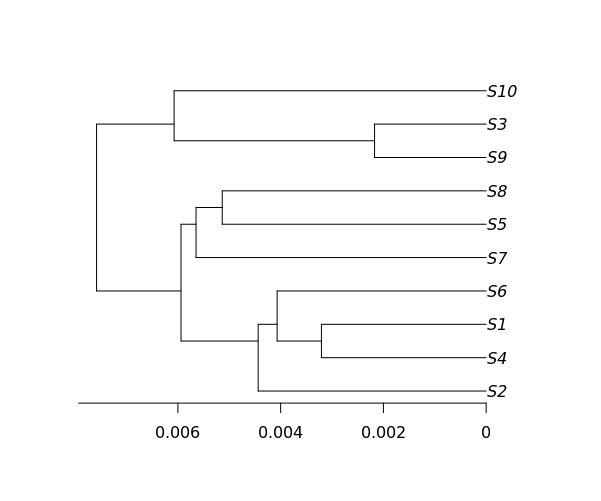
\includegraphics[width=0.5\textwidth]{plots/Coalescent_Example.png}
    \caption{An example simulated coalescent tree}
\end{figure}

\begin{lstlisting}
f <- (sampling_times, Ne): //Sampling times in descending order
  extant_lineages <- 1
  future_lineages <- length(sampling_times)-1
  t <- sampling_times[1]
  idx <- 1
  log_lh <- 0

  while extant_lineages > 1 or future_lineages > 0:
    if extant_lineages < 2:
      idx++
      t <- sampling_times[idx]
      extant_lineages++
      future_lineages--
    else:
      delta_t <- t-sampling_times[idx+1]
      rate <- binom(extant_lineages,2)/Ne

      p_coal <- 1-exp(-rate*delta_t)
      r_c ~ U[0,1] 

      if r_c < p_coal:

        log_lh += log(p_coal)

        coalesce_lineages
        extant_lineages--

        r_w ~ U[0,1]
        w_t <- (-1/rate)*log(1-r_w*(1-exp(-rate*delta_t)))
        t <- t+w_t

        cond_lh <- rate*(1/(1-exp(-rate*delta_t)) - r_w)
        log_lh += log(cond_lh)

      else:
        log_lh += log(1-p_coal)
        idx++
        t <- sampling_times[idx]
        extant_lineages++
        future_lineages--

    return: coalescent_times, log_lh
\end{lstlisting}

\subsection{Inhomogenous Case}
In the inhomogenous case, the scheme is similar, with the key difference that the sampling times now follow a much more complex distribution. As such a sampling scheme such as rejection sampling will be required (?)
\subsection{Multistrain+Inhomogenous Case}
In this case, coalescent nodes have an added colour property, and each colour coalesces according to a colour specific, time dependent case. Nodes of non-identical colour can coalesce iff at least one of them is the last remaining node of a given colour.\\
Given $M$ colours, $M$ population size functions $\{Ne_j(t)\}_{1\leq j\leq M}$, and initial population size $N$, Let $Y(t)$ be a CTMC with the state space:
\begin{gather}
  S = \left\{\mathbf{s}\in \Z_+^{N}:|\mathbf{s}|\leq N, |\mathbf{s}|\geq1\right\}
\end{gather}
and the transition rates
\begin{gather}
\mathbf{s}\to\mathbf{s}-\mathbf{e_j} \quad \binom{s_j}{2}Ne_j(t)+\delta_{s_j, 1}Ne_j(t)\sum_{i\neq j}s_i
\end{gather}

\section{Previous Work}
A framework utilising sampling intensity in order to extract more information is proposed in \cite{parag_jointly_nodate}
\section{Bibliography}
\printbibliography
\end{document}
